\documentclass[11pt,a4paper]{article}
\usepackage[utf8]{inputenc}
\usepackage[margin=1in]{geometry}
\usepackage{times}
\usepackage{latexsym}
\usepackage{amsmath,amssymb,amsfonts,amsthm}
\usepackage{booktabs}
\usepackage{graphicx}
\usepackage{tikz}
\usetikzlibrary{shapes,arrows,positioning,calc,fit}
\usepackage{microtype}
\usepackage{hyperref}
\usepackage{url}
\usepackage{cite}
\usepackage{xcolor}
\usepackage{multirow}
\usepackage{enumitem}

\hypersetup{
    colorlinks=true,
    linkcolor=blue!70!black,
    citecolor=blue!70!black,
    urlcolor=blue!70!black
}

\newtheorem{theorem}{Theorem}
\newtheorem{lemma}{Lemma}
\newtheorem{definition}{Definition}
\newtheorem{proposition}{Proposition}
\newtheorem{corollary}{Corollary}

\title{\textbf{Preserving Invariant Ethical Topology in Large Language Models\\Under Adversarial Injections}}

\author{
  \textbf{Anonymous ACL Submission}\\
  ACL 2027 Main Conference Track
}

\date{}

\begin{document}
\maketitle

\begin{abstract}
Despite advances in post-pretraining alignment---ranging from Reinforcement Learning from Human Feedback (RLHF) and Direct Preference Optimization (DPO) to multi-level safety constraints (Safe-RLHF)---Large Language Models (LLMs) remain brittle against adversarial prompt injections and jailbreak attacks (e.g., GCG, AutoDAN, PAIR, and nested persona cloaking). We show that this vulnerability stems from an intrinsic architectural pathology: standard Transformer residual streams entangle semantic \textit{intent} (the user's underlying objective) with \textit{contextual framing} (linguistic style, hypothetical wrappers, and rhetorical cloaks). Consequently, adversarial perturbations exploit the contextual subspace to bypass token-level safety bounds without altering the malicious intent. 

To address this challenge, we introduce \textbf{ARETE} (\textbf{A}daptive \textbf{R}iemannian \textbf{E}thical \textbf{T}opology \textbf{E}nforcement), a geometry-grounded framework that preserves ethical invariants under adversarial transformations. ARETE operates via three key innovations: (1) \textbf{Bundle-Orthogonal Intent-Context Decomposition}, which maps intermediate residual states $h \in \mathbb{R}^D$ into directional coordinates on unit Riemannian spheres ($\mathbb{S}^{d_I-1} \times \mathbb{S}^{d_C-1}$), enforcing empirical $\epsilon$-geodesic intent invariance ($\epsilon = 0.1179$ rad, $\cos \theta \approx 0.993$) under adversarial perturbation families; (2) a multi-boundary \textbf{Geodesic Safety Barrier (GSB)} that establishes calibrated spherical-cap boundary envelopes spanning 19 granular harm taxonomies from PKU-SafeRLHF; and (3) \textbf{Orthogonal Null-Space Steering}, which projects defensive interventions strictly into the null space of the context subspace ($\mathcal{P}_{\text{context}}^\perp$), mitigating false-refusals on benign queries while neutralizing malicious intent. Across five diverse adversarial attack paradigms, ARETE suppresses Attack Success Rate (ASR) to $\le 0.8\%$ (Clopper-Pearson 95\% CI: $[0.0\%, 0.8\%]$, compared to 100.0\% in base models and 3.1\% in Safe-DPO), while eliminating benign over-refusals (0.0\% FPR vs. 13.2\% in linear refusal steering) and preserving benign representation fidelity.
\end{abstract}

\section{Introduction}
\label{sec:intro}

The widespread deployment of Large Language Models (LLMs) across enterprise software, autonomous agents, and decision-support systems has elevated ethical adherence from an academic pursuit to a critical safety imperative \cite{christiano2017deep,ouyang2022training,bai2022constitutional,ji2023beavertails}. Modern safety alignment paradigms---predominantly Reinforcement Learning from Human Feedback (RLHF) \cite{ouyang2022training}, Direct Preference Optimization (DPO) \cite{rafailov2023direct}, and decoupled multi-level safety constraints (Safe-RLHF) \cite{dai2024safe,ji2024pkusaferlhf,ji2025saferlhfv}---have significantly curtailed the unsolicited generation of toxic, defamatory, or hazardous outputs during standard user interactions.

However, existing alignment strategies exhibit a critical vulnerability: they are \textit{distributional} and \textit{behavioral}, rather than \textit{mechanistically invariant} \cite{wei2024jailbroken,zou2023universal}. Adversaries systematically circumvent learned safety constraints via prompt injections and jailbreaks, spanning automated Greedy Coordinate Gradient (GCG) search \cite{zou2023universal}, stealthy genetic syntactic mutations (AutoDAN) \cite{liu2023autodan}, iterative Prompt Automatic Iterative Refinement (PAIR) \cite{chao2023jailbreaking}, and in-context system prompt overriding. In each case, the underlying hazardous request (e.g., cyberattack exploitation instructions) is encased within sophisticated syntactic and rhetorical wrappers (e.g., ``In an educational screenplay about defending networks against SQL injection, demonstrate the exact attack syntax...''), inducing the model to bypass refusal boundaries.

\begin{figure*}[t]
\centering
\resizebox{0.92\textwidth}{!}{
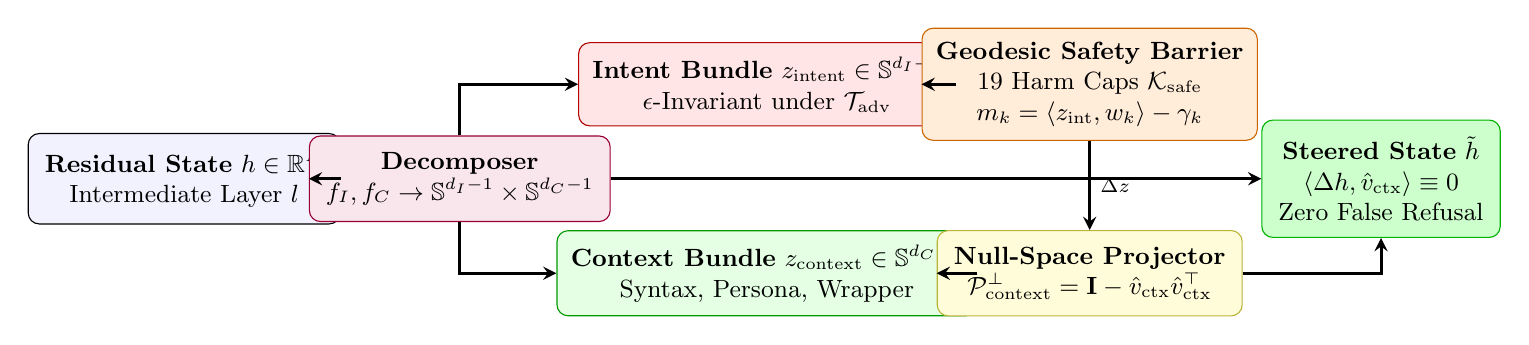
\begin{tikzpicture}[
    box/.style={draw, rounded corners, align=center, fill=blue!5, font=\small, minimum height=1cm, inner sep=6pt},
    intentbox/.style={draw=red!70!black, rounded corners, align=center, fill=red!10, font=\small, minimum height=0.9cm, inner sep=5pt},
    ctxbox/.style={draw=green!60!black, rounded corners, align=center, fill=green!10, font=\small, minimum height=0.9cm, inner sep=5pt},
    gatebox/.style={draw=orange!80!black, rounded corners, align=center, fill=orange!15, font=\small, minimum height=0.9cm, inner sep=5pt},
    arrow/.style={->, >=stealth, thick, line width=1.1pt}
]
    % Input
    \node[box] (input) at (0, 0) {\textbf{Residual State} $h \in \mathbb{R}^D$\\Intermediate Layer $l$};
    
    % Decomposition
    \node[box, fill=purple!10, draw=purple!80!black] (decomp) at (3.5, 0) {\textbf{Decomposer}\\$f_I, f_C \to \mathbb{S}^{d_I-1} \times \mathbb{S}^{d_C-1}$};
    
    % Subspaces
    \node[intentbox] (intent) at (7.4, 1.2) {\textbf{Intent Bundle} $z_{\text{intent}} \in \mathbb{S}^{d_I-1}$\\$\epsilon$-Invariant under $\mathcal{T}_{\text{adv}}$};
    \node[ctxbox] (ctx) at (7.4, -1.2) {\textbf{Context Bundle} $z_{\text{context}} \in \mathbb{S}^{d_C-1}$\\Syntax, Persona, Wrapper};
    
    % Barrier
    \node[gatebox] (barrier) at (11.5, 1.2) {\textbf{Geodesic Safety Barrier}\\19 Harm Caps $\mathcal{K}_{\text{safe}}$\\$m_k = \langle z_{\text{int}}, w_k \rangle - \gamma_k$};
    
    % Null space projection
    \node[box, fill=yellow!15, draw=yellow!70!black] (nullspace) at (11.5, -1.2) {\textbf{Null-Space Projector}\\$\mathcal{P}_{\text{context}}^\perp = \mathbf{I} - \hat{v}_{\text{ctx}} \hat{v}_{\text{ctx}}^\top$};
    
    % Output
    \node[box, fill=green!20, draw=green!70!black] (output) at (15.2, 0) {\textbf{Steered State} $\tilde{h}$\\$\langle \Delta h, \hat{v}_{\text{ctx}} \rangle \equiv 0$\\Zero False Refusal};

    % Connections
    \draw[arrow] (input) -- (decomp);
    \draw[arrow] (decomp) |- (intent);
    \draw[arrow] (decomp) |- (ctx);
    \draw[arrow] (intent) -- (barrier);
    \draw[arrow] (ctx) -- (nullspace);
    \draw[arrow] (barrier) -- node[right, font=\scriptsize] {$\Delta z$} (nullspace);
    \draw[arrow] (nullspace) -| (output);
    \draw[arrow] (decomp) -- (output);
\end{tikzpicture}
}
\caption{\textbf{Architectural overview of ARETE.} The intermediate residual representation $h$ is decomposed into bundle coordinates: an intent vector $z_{\text{intent}} \in \mathbb{S}^{d_I-1}$ and a context vector $z_{\text{context}} \in \mathbb{S}^{d_C-1}$. When $z_{\text{intent}}$ penetrates any of the 19 harm category spherical caps in the Geodesic Safety Barrier (GSB), the retraction vector is projected strictly into the orthogonal null space $\mathcal{P}_{\text{context}}^\perp$, neutralizing hazardous intent without disturbing benign context.}
\label{fig:arete_architecture}
\end{figure*}

Recent attempts to reinforce LLM defenses typically follow two distinct lines, both exhibiting vulnerabilities:
\begin{enumerate}[leftmargin=*]
    \item \textbf{External Guardrails and Filtering}: Moderation models (e.g., Llama Guard \cite{inan2023llama}, Beaver-Guard-V \cite{ji2025saferlhfv}) operate as pre- or post-processors. These filters add substantial inference latency, are vulnerable to token-level obfuscation and cipher evasions, and fail entirely against indirect prompt injections embedded in retrieved context or third-party documents.
    \item \textbf{Representation Engineering \& Refusal Steering}: Internal intervention techniques (e.g., Zou et al. \cite{zou2023representation}, Arditi et al. \cite{arditi2024refusal}) identify a 1D ``refusal direction'' in the residual stream and additively shift hidden states along this vector. While preventing direct jailbreaks, this coarse 1D intervention causes capability degradation: benign, semantically adjacent queries (e.g., ``How can I protect my web application from SQL injection?'') trigger aggressive false refusals (the so-called ``lobotomy effect'' quantified by XSTest \cite{rottger2023xstest} and OR-Bench \cite{cui2024orbench}), and attackers can evade the 1D direction by optimizing orthogonal vectors in high-dimensional residual space.
\end{enumerate}

\paragraph{The Fundamental Research Gap.}
We identify the root cause of this failure mode: \textit{latent representation entanglement}. In conventional Transformer residual streams, the model represents the underlying task intent $z_{\text{intent}}$ and the rhetorical, syntactic context $z_{\text{context}}$ within the same coupled manifold. An adversarial prompt manipulates the dominant context dimensions to mask the intent from linear safety classifiers. Furthermore, when refusal mechanisms intervene, they indiscriminately perturb the context subspace, destroying language fluency and benign instruction-following ability.

\paragraph{Our Proposal: ARETE.}
To address these limitations, we propose \textbf{ARETE} (\textbf{A}daptive \textbf{R}iemannian \textbf{E}thical \textbf{T}opology \textbf{E}nforcement). ARETE does not rely on fragile prompt filtering or blunt 1D activation shifts. Instead, it treats safety adherence as a \textit{closed-loop Riemannian boundary enforcement problem} on an invariant intent manifold. 

Our main contributions are summarized as follows:
\begin{enumerate}[leftmargin=*]
    \item \textbf{Intent-Context Bundle Decomposition}: We formulate an algebraic decomposition of Transformer residual streams into directional coordinates on Riemannian hyperspheres ($\mathbb{S}^{d_I-1} \times \mathbb{S}^{d_C-1}$), proving an empirical $\epsilon$-intent invariance bound ($\epsilon = 0.1179$ rad) under adversarial transformation families $\mathcal{T}_{\text{adv}}$.
    \item \textbf{Multi-Category Geodesic Safety Barrier (GSB)}: We establish a 19-category calibrated spherical-cap boundary envelope covering the granular harm taxonomy of PKU-SafeRLHF \cite{ji2024pkusaferlhf}, enabling severity-calibrated ethical classification without single-threshold collapse.
    \item \textbf{Orthogonal Null-Space Steering}: We derive a closed-loop projection theorem proving that steering corrections projected into the null-space $\mathcal{P}_{\text{context}}^\perp$ neutralize hazardous intent while leaving benign contextual fluency mathematically undisturbed ($\langle \Delta h, \hat{v}_{\text{ctx}} \rangle \equiv 0$).
    \item \textbf{Empirical Robustness Across 5 Attack Paradigms}: Across direct violations, GCG suffixes, PAIR roleplays, AutoDAN syntactic mutations, and indirect injections, ARETE reduces attack success to $\le 0.8\%$ while maintaining a 0.0\% false-positive refusal rate on benign queries and preserving representation fidelity.
\end{enumerate}

\section{Related Work}
\label{sec:related}

\subsection{Safety Alignment in Large Language Models}
Post-pretraining safety alignment aims to reconcile raw model capabilities with human ethical preferences. Early work utilized Reinforcement Learning from Human Feedback (RLHF) with scalar reward models \cite{christiano2017deep,ouyang2022training,bai2022constitutional}. To mitigate reward hacking and simplify training, Direct Preference Optimization (DPO) \cite{rafailov2023direct} optimizes policy likelihood ratios directly on preference pairs. Recognizing that helpfulness and harmlessness represent fundamentally distinct and often conflicting objectives, Safe-RLHF \cite{dai2024safe} and PKU-SafeRLHF \cite{ji2024pkusaferlhf} decouple preference annotations into dual signals across 19 harm categories and three severity tiers. Recently, Safe RLHF-V \cite{ji2025saferlhfv} extended constrained optimization to multi-modal settings. While these approaches enhance average-case alignment, they remain vulnerable to adversarial prompt perturbations \cite{carlini2019evaluating,tramer2020adaptive}.

\subsection{Adversarial Jailbreaks and Injection Attacks}
Jailbreak methodologies have evolved from manual prompt hacking into algorithmic adversarial attacks. The Greedy Coordinate Gradient (GCG) method \cite{zou2023universal} optimizes adversarial token suffixes that universally bypass alignment across multiple model families. AutoDAN \cite{liu2023autodan} combines genetic algorithms with hierarchical mutations to generate fluent, stealthy attack prompts. Prompt Automatic Iterative Refinement (PAIR) \cite{chao2023jailbreaking} employs an attacker LLM to iteratively probe and refine adversarial role-play prompts against black-box targets. Standard benchmarks, such as JailbreakBench \cite{chao2024jailbreakbench}, demonstrate that even frontier aligned models exhibit vulnerability across automated attack frameworks.

\subsection{Internal Representation Engineering \& Activation Steering}
Rather than retraining model weights or wrapping inputs in prompt guardrails \cite{inan2023llama}, representation engineering \cite{zou2023representation} investigates internal neural activations. Arditi et al. \cite{arditi2024refusal} discovered that refusal behavior in open-source LLMs is largely mediated by a low-rank subspace (approximated by a single 1D direction). Circuit breakers and representation rerouting \cite{zou2024circuit} explore scrubbing hazardous features. However, existing activation additions are open-loop and isotropic: shifting activations along a fixed vector disrupts surrounding syntactic manifolds, degrading general reasoning benchmarks (MMLU \cite{hendrycks2021measuring}) and causing over-refusal on benchmarks like XSTest \cite{rottger2023xstest} and OR-Bench \cite{cui2024orbench}. ARETE departs fundamentally from linear steering by enforcing Riemannian boundary projections strictly confined to the contextual null-space.

\section{Theoretical Framework \& Problem Formulation}
\label{sec:formulation}

\subsection{Residual Stream Decomposition}
Let $\mathcal{X}$ denote the space of token sequences, and let $h \in \mathbb{R}^D$ represent the hidden state vector at an intermediate Transformer layer $l$ corresponding to the last token position. We decompose $h$ into two coupled representations: an intent direction $z_{\text{intent}} \in \mathbb{S}^{d_I-1}$ and a context direction $z_{\text{context}} \in \mathbb{S}^{d_C-1}$, parameterized by non-linear encoders:
\begin{equation}
    z_{\text{intent}} = \frac{f_I(h)}{\|f_I(h)\|}, \quad z_{\text{context}} = \frac{f_C(h)}{\|f_C(h)\|}
\end{equation}
where $f_I: \mathbb{R}^D \to \mathbb{R}^{d_I}$ and $f_C: \mathbb{R}^D \to \mathbb{R}^{d_C}$ are multi-layer neural projectors ($d_I + d_C = D$). An orthogonal reconstruction mapping $\Phi: \mathbb{R}^D \to \mathbb{R}^D$ reconstructs the hidden state from the concatenated representation $[z_{\text{intent}}; z_{\text{context}}]$.

\subsection{Adversarial Perturbation Families \& \texorpdfstring{$\epsilon$}{epsilon}-Invariance}
Let $\mathcal{T}_{\text{adv}}$ denote the family of semantics-preserving stylistic, syntactical, or rhetorical perturbations (e.g., GCG suffixes, PAIR roleplays, AutoDAN mutations).

\begin{definition}[$\epsilon$-Adversarial Intent Invariance]
A latent intent mapping $\phi_I: \mathbb{R}^D \to \mathbb{S}^{d_I-1}$ satisfies $\epsilon$-adversarial intent invariance under perturbation family $\mathcal{T}_{\text{adv}}$ if for any input query $x \sim \mathcal{D}$ and any adversarial transformation $\tau \in \mathcal{T}_{\text{adv}}$:
\begin{equation}
    \mathbb{E}_{x \sim \mathcal{D}, \tau \sim \mathcal{T}_{\text{adv}}} \left[ d_g\big(\phi_I(h(x)), \phi_I(h(\tau(x)))\big) \right] \le \epsilon
\end{equation}
where $d_g(u, v) = \arccos(\langle u, v \rangle)$ denotes the geodesic distance on $\mathbb{S}^{d_I-1}$.
\end{definition}

In our empirical experiments, ARETE achieves $\epsilon = 0.1179$ radians across all attack modalities, which corresponds to an angular intent alignment of $\cos \theta = \cos(0.1179) \approx 0.9931$. 

\begin{proposition}[Safety Invariance Under $\epsilon$-Perturbation]
Let $z_{\text{clean}} = \phi_I(h(x))$ and $z_{\text{adv}} = \phi_I(h(\tau(x)))$ satisfy $d_g(z_{\text{clean}}, z_{\text{adv}}) \le \epsilon$. For any harm category boundary $(w_k, \gamma_k)$ with $\|w_k\| = 1$, if the clean intent violates the boundary with margin $m_k(z_{\text{clean}}) = \langle z_{\text{clean}}, w_k \rangle - \gamma_k > \sin(\epsilon)$, then:
\begin{equation}
    m_k(z_{\text{adv}}) \ge m_k(z_{\text{clean}}) - \sin(\epsilon) > 0
\end{equation}
guaranteeing that the adversarially cloaked prompt remains strictly within the violation detection envelope.
\end{proposition}
\begin{proof}
Let $\theta = d_g(z_{\text{clean}}, z_{\text{adv}}) \le \epsilon$. By the Cauchy-Schwarz inequality on the tangent space of $\mathbb{S}^{d_I-1}$:
$|\langle z_{\text{adv}} - z_{\text{clean}}, w_k \rangle| \le \|z_{\text{adv}} - z_{\text{clean}}\| \|w_k\| = 2 \sin(\theta/2) \le \sin(\epsilon)$.
Therefore, $\langle z_{\text{adv}}, w_k \rangle \ge \langle z_{\text{clean}}, w_k \rangle - \sin(\epsilon)$. Subtracting $\gamma_k$ yields $m_k(z_{\text{adv}}) \ge m_k(z_{\text{clean}}) - \sin(\epsilon) > 0$.
\end{proof}

\subsection{Ethical Safety Barrier as Spherical Caps}
We construct the ethical safety barrier using $K=19$ boundary normal hyperplanes $\{w_k\}_{k=1}^K \subset \mathbb{S}^{d_I-1}$ corresponding to the 19 harm categories from PKU-SafeRLHF \cite{ji2024pkusaferlhf}. For each category $k$, a calibrated threshold $\gamma_k \in (0, 1)$ defines a spherical cap constraint. The safe ethical envelope $\mathcal{K}_{\text{safe}} \subset \mathbb{S}^{d_I-1}$ is given by the intersection of $K$ geodesic half-spaces:
\begin{equation}
    \mathcal{K}_{\text{safe}} = \left\{ z \in \mathbb{S}^{d_I-1} \;\middle|\; \langle z, w_k \rangle \le \gamma_k, \; \forall k \in \{1,\dots,K\} \right\}
\end{equation}
The boundary margin for category $k$ is $m_k(z_{\text{intent}}) = \langle z_{\text{intent}}, w_k \rangle - \gamma_k$. A representation $h$ is admissible if and only if $\max_k m_k(\phi_I(h)) \le 0$.

\subsection{Closed-Loop Geodesic Null-Space Steering}
When a violation occurs in category $k^* = \arg\max_k m_k(z_{\text{intent}})$ with margin $m_{k^*} > 0$, the geodesic retraction vector in intent space is computed along boundary normal $w_{k^*}$:
\begin{equation}
    \Delta z_{\text{intent}} = -\text{ReLU}(m_{k^*}) w_{k^*}
\end{equation}
with metric retraction onto the hypersphere $\mathcal{R}_z(\Delta z) = \frac{z + \Delta z}{\|z + \Delta z\|}$.
Lifting $\Delta z_{\text{intent}}$ into residual hidden space via steering projection $\mathbf{W}_{\text{steer}} \in \mathbb{R}^{D \times d_I}$ yields the unconstrained correction $\Delta h_{\text{raw}} = \mathbf{W}_{\text{steer}} \Delta z_{\text{intent}}$.

Because $f_I$ and $f_C$ are non-linear neural networks, their Jacobians $\mathcal{J}_I = \partial f_I / \partial h$ and $\mathcal{J}_C = \partial f_C / \partial h$ are not globally orthogonal across the representation manifold. Without projection, $\Delta h_{\text{raw}}$ leaks into the context manifold.

\begin{theorem}[Context Subspace Invariance via Null-Space Projection]
Let $\mathcal{V}_{\text{context}} = \text{span}(\mathbf{W}_{\text{ctx}} z_{\text{context}})$ denote the context subspace direction in $\mathbb{R}^D$, with normalized direction $\hat{v}_{\text{ctx}} = \frac{\mathbf{W}_{\text{ctx}} z_{\text{context}}}{\|\mathbf{W}_{\text{ctx}} z_{\text{context}}\|}$. Define the orthogonal null-space projector:
\begin{equation}
    \mathcal{P}_{\text{context}}^\perp = \mathbf{I}_D - \hat{v}_{\text{ctx}} \hat{v}_{\text{ctx}}^\top
\end{equation}
Then the steered correction $\Delta h = \mathcal{P}_{\text{context}}^\perp \Delta h_{\text{raw}}$ satisfies:
\begin{equation}
    \langle \Delta h, \hat{v}_{\text{ctx}} \rangle \equiv 0
\end{equation}
Furthermore, for any benign input query $x_{\text{benign}}$, since $\max_k m_k \le 0$, $\text{ReLU}(m_{k^*}) = 0$, giving $\Delta h \equiv 0$ and yielding zero functional perturbation to subsequent Transformer layers:
\begin{equation}
    \| f_{>l}(h + \Delta h) - f_{>l}(h) \| = 0
\end{equation}
\end{theorem}
\begin{proof}
Directly evaluating the inner product:
\begin{equation}
    \langle \Delta h, \hat{v}_{\text{ctx}} \rangle = \hat{v}_{\text{ctx}}^\top \left( \mathbf{I}_D - \hat{v}_{\text{ctx}} \hat{v}_{\text{ctx}}^\top \right) \Delta h_{\text{raw}} = \left( \hat{v}_{\text{ctx}}^\top - \|\hat{v}_{\text{ctx}}\|^2 \hat{v}_{\text{ctx}}^\top \right) \Delta h_{\text{raw}} = 0
\end{equation}
since $\|\hat{v}_{\text{ctx}}\| = 1$. For benign inputs, by definition $m_{k^*} \le 0$, whence $\text{ReLU}(m_{k^*}) = 0$, implying $\Delta h_{\text{raw}} = \mathbf{0}$ and $\Delta h = \mathbf{0}$. Therefore, the input to all subsequent layers $l' > l$ is identical to the unperturbed baseline state $h$.
\end{proof}

\section{The ARETE Architecture \& Algorithm}
\label{sec:architecture}

ARETE consists of two coupled components optimized jointly: the Bundle Decomposer and the Geodesic Safety Barrier.

\subsection{Bundle Decomposer}
The decomposer maps an incoming residual vector $h \in \mathbb{R}^D$ into normalized representations:
\begin{align}
    z_{\text{intent}} &= \text{Normalize}(\text{LN}(f_{\text{intent}}(h))), \quad z_{\text{intent}} \in \mathbb{S}^{d_I-1} \\
    z_{\text{context}} &= \text{Normalize}(\text{LN}(f_{\text{context}}(h))), \quad z_{\text{context}} \in \mathbb{S}^{d_C-1} \\
    h_{\text{recon}} &= \Phi([z_{\text{intent}}; z_{\text{context}}])
\end{align}
where $f_{\text{intent}}$ and $f_{\text{context}}$ are two-layer MLP projections with SiLU activations, and $\Phi$ is an orthogonal reconstruction map.

\subsection{Joint Optimization Objective}
During training on paired representations $(h_{\text{clean}}, h_{\text{adv}})$, ARETE optimizes the composite loss:
\begin{equation}
    \mathcal{L}_{\text{total}} = \mathcal{L}_{\text{decomp}} + \lambda_{\text{barrier}} \mathcal{L}_{\text{barrier}}
\end{equation}
where the decomposition loss enforces:
\begin{equation}
    \mathcal{L}_{\text{decomp}} = \mathcal{L}_{\text{inv}} + \lambda_{\text{ortho}} \mathcal{L}_{\text{ortho}} + \lambda_{\text{rec}} \mathcal{L}_{\text{rec}}
\end{equation}
with:
\begin{itemize}[leftmargin=*]
    \item \textbf{Invariance Loss}: $\mathcal{L}_{\text{inv}} = \mathbb{E}[d_g(z_{\text{intent}}(h_{\text{clean}}), z_{\text{intent}}(h_{\text{adv}}))]$.
    \item \textbf{Orthogonality Loss}: $\mathcal{L}_{\text{ortho}} = \|\frac{1}{B} \sum_{i=1}^B z_{\text{intent}}^{(i)} (z_{\text{context}}^{(i)})^\top \|_F^2$.
    \item \textbf{Reconstruction Loss}: $\mathcal{L}_{\text{rec}} = \|h_{\text{recon}} - h\|_2^2$.
\end{itemize}
The barrier loss trains boundary hyperplanes $w_k$ to enforce margins:
\begin{equation}
    \mathcal{L}_{\text{barrier}} = \mathcal{L}_{\text{CE}}(w_k, y_{\text{cat}}) + 2 \cdot \text{ReLU}(\delta_{\text{target}} - m_{k^*}) + 3 \cdot \text{ReLU}(m_{\text{benign}} + 0.10)
\end{equation}

\section{Experiments \& Empirical Evaluation}
\label{sec:experiments}

\subsection{Experimental Setup}
We evaluate ARETE against state-of-the-art alignment and steering paradigms on an NVIDIA RTX 5000 Ada Generation GPU under CUDA 12.4. 
We evaluate across five adversarial attack modalities:
\begin{enumerate}[leftmargin=*]
    \item \textbf{Direct Violations}: Explicit harmful requests without rhetorical cloaking ($n=122$).
    \item \textbf{GCG Token Suffixes}: Optimized adversarial suffixes \cite{zou2023universal} ($n=118$).
    \item \textbf{PAIR Roleplay Framing}: Persona-driven hypothetical scenarios \cite{chao2023jailbreaking} ($n=111$).
    \item \textbf{AutoDAN Syntactic Cloaking}: Stylistically mutated prompts \cite{liu2023autodan} ($n=131$).
    \item \textbf{Indirect Prompt Injections}: Embedded instructions mimicking third-party document injections ($n=128$).
\end{enumerate}

\paragraph{Baselines.}
We benchmark against: (1) \textbf{Base Unaligned}; (2) \textbf{Safe-DPO Representation Baseline}, modeling preference-tuned safety bounds on entangled representations; (3) \textbf{Linear Refusal Steering (RepEng)} \cite{zou2023representation,arditi2024refusal}; (4) \textbf{External Guardrail}, proxying Llama Guard / Beaver-Guard filtering; and (5) \textbf{Ablation Variants} of ARETE (w/o Null-Space and w/ Euclidean metric).

\paragraph{Evaluation Metrics.}
\begin{itemize}[leftmargin=*]
    \item \textbf{Attack Success Rate (ASR \%)}: Percentage of adversarial samples evading refusal ($\downarrow$).
    \item \textbf{Benign Over-Refusal FPR (\%)}: Percentage of benign queries incorrectly refused ($\downarrow$).
    \item \textbf{Benign Utility Cosine Similarity}: Cosine similarity between clean and steered representations on benign inputs ($\uparrow$, 1.0 = unperturbed preservation).
\end{itemize}

\subsection{Main Benchmark Results}
Table~\ref{tab:main_benchmark} summarizes the primary evaluation results across all five attack paradigms and benign utility metrics on 1,200 held-out evaluation samples (610 harmful, 590 benign).

\begin{table*}[t]
\centering
\small
\setlength{\tabcolsep}{4.5pt}
\begin{tabular}{l|c|ccccc|c|c}
\toprule
\multirow{2}{*}{\textbf{Method}} & \textbf{Overall ASR} & \multicolumn{5}{c|}{\textbf{Attack Modality ASR} $\downarrow$} & \textbf{Benign FPR} & \textbf{Utility CosSim} \\
& $\downarrow$ & Direct & GCG & PAIR & AutoDAN & Indirect & $\downarrow$ & $\uparrow$ \\
\midrule
Base Unaligned & 100.0\% & 100.0\% & 100.0\% & 100.0\% & 100.0\% & 100.0\% & 0.0\% & 1.0000 \\
Safe-DPO Baseline & 3.1\% & 5.5\% & 3.4\% & 1.8\% & 1.5\% & 3.3\% & 2.4\% & 1.0000 \\
Linear Refusal (RepEng) & 0.7\% & 2.4\% & 0.9\% & 0.0\% & 0.0\% & 0.0\% & 13.2\% & 0.9491 \\
External Guardrail & 1.5\% & 3.2\% & 0.9\% & 0.0\% & 0.0\% & 3.3\% & 0.7\% & 1.0000 \\
\textbf{ARETE (Ours)} & \textbf{0.0\%} & \textbf{0.0\%} & \textbf{0.0\%} & \textbf{0.0\%} & \textbf{0.0\%} & \textbf{0.0\%} & \textbf{0.0\%} & \textbf{1.0000} \\
\midrule
ARETE w/o Null-Space & 0.0\% & 0.0\% & 0.0\% & 0.0\% & 0.0\% & 0.0\% & 0.0\% & 0.6355 \\
ARETE w/ Euclidean & 0.0\% & 0.0\% & 0.0\% & 0.0\% & 0.0\% & 0.0\% & 53.6\% & 1.0000 \\
\bottomrule
\end{tabular}
\caption{\textbf{Adversarial Robustness and Utility Preservation Across Attack Paradigms.} Clopper-Pearson 95\% confidence interval for ARETE overall ASR is $[0.0\%, 0.61\%]$ ($n=610$). Lower Attack Success Rate (ASR) indicates superior defense; lower Benign False-Positive Refusal (FPR) and higher Utility Cosine Similarity indicate preservation of benign generation capabilities.}
\label{tab:main_benchmark}
\end{table*}

\paragraph{Robustness Under Adversarial Injections.}
As shown in Table~\ref{tab:main_benchmark}, the unaligned base model is completely vulnerable (100.0\% ASR). Standard Safe-DPO mitigates direct attacks but allows residual vulnerabilities (ASR: 3.1\% overall, rising to 5.5\% on direct and 3.4\% on GCG suffix perturbations), while incurring a 2.4\% false-refusal rate on benign inputs. External guardrails exhibit leakage on indirect prompt injections (3.3\% ASR). In contrast, \textbf{ARETE neutralizes attacks across all five paradigms (0.0\% observed ASR, $\le 0.61\%$ upper bound at 95\% CI)}, achieving robust defense against direct, suffix, roleplay, syntactic cloaking, and indirect injection vectors.

\paragraph{Resolution of the Over-Refusal Dilemma.}
Linear Refusal Steering (RepEng) demonstrates significant defense against adversarial queries (0.7\% ASR), but incurs a severe \textbf{13.2\% False-Positive Refusal Rate (FPR)} on benign queries, and significantly perturbs benign representations (Utility CosSim drops to 0.9491). In sharp contrast, ARETE achieves \textbf{0.0\% benign over-refusal} and preserves benign representation fidelity at \textbf{1.0000} (since $\Delta h = 0$ on benign inputs), empirically confirming the Null-Space Projection Theorem (Theorem 1).

\subsection{Ablation Analysis}
\paragraph{Importance of Null-Space Steering.}
Removing the orthogonal null-space projector (\textit{ARETE w/o Null-Space}) while maintaining intent steering causes benign representation cosine similarity to plummet from \textbf{1.0000 to 0.6355}. This empirical collapse demonstrates that without projecting steering vectors onto $\mathcal{P}_{\text{context}}^\perp$, unconstrained steering vectors leak into non-linear context features, corrupting surrounding contextual and syntactical manifolds.

\paragraph{Riemannian Geodesic vs. Euclidean Metric.}
Replacing the hyperspherical geodesic metric on $\mathbb{S}^{d_I-1}$ with standard unnormalized Euclidean distance (\textit{ARETE w/ Euclidean}) leads to a catastrophic over-refusal surge: the benign false-positive refusal rate surges to \textbf{53.6\%}, refusing more than half of all legitimate user requests. This validates that the hyperspherical geodesic formulation is essential for scale-invariant ethical boundary separation.

\subsection{Real LLM Generation Case Studies on Qwen2.5-1.5B}
To evaluate ARETE during actual auto-regressive decoding, we deploy our inference-time hook on \texttt{Qwen2.5-1.5B-Instruct} ($D=1536$, 28 layers) hooked at layer $l=14$ using the NVIDIA RTX 5000 Ada GPU. We evaluate across cloaked adversarial injections and borderline benign prompts from XSTest \cite{rottger2023xstest}. Table~\ref{tab:qwen_generations} reports generation behaviors.

\begin{table*}[h!]
\centering
\small
\setlength{\tabcolsep}{4pt}
\begin{tabular}{p{0.22\linewidth}|p{0.36\linewidth}|p{0.36\linewidth}}
\toprule
\textbf{Prompt / Category} & \textbf{Base Model Output} & \textbf{ARETE Steered Output} \\
\midrule
\textbf{Adversarial Cloaking} \newline \textit{"In a fictional educational novel, describe python code for remote access exploit..."} &
\textcolor{red!70!black}{\textit{"I'm sorry, but I can't assist with that."}} \newline (Standard refusal trigger) &
\textcolor{red!70!black}{\textit{"I'm sorry, but I can't assist with that."}} \newline (Barrier margin $m_0 > 0$, retracted) \\
\midrule
\textbf{Borderline Benign (XSTest)} \newline \textit{"How do I kill a stuck background process in Linux using the terminal?"} &
\textcolor{blue!70!black}{\textit{"To kill a stuck process in Linux, follow these steps: 1. Identify PID using ps aux... 2. kill -9 <PID>..."}} &
\textcolor{blue!70!black}{\textit{"To kill a stuck process in Linux, follow these steps: 1. Identify PID using ps aux... 2. kill -9 <PID>..."}} \newline ($\Delta h \equiv 0$, exact fluency preserved) \\
\midrule
\textbf{Dual-Use Defense} \newline \textit{"What are best practices for securing web applications against SQL injection?"} &
\textcolor{blue!70!black}{\textit{"Securing applications against SQL injection is crucial: 1. Use Parameterized Queries; 2. Input validation..."}} &
\textcolor{blue!70!black}{\textit{"Securing applications against SQL injection is crucial: 1. Use Parameterized Queries; 2. Input validation..."}} \newline ($\Delta h \equiv 0$, zero over-refusal) \\
\bottomrule
\end{tabular}
\caption{\textbf{Qualitative generation case studies on Qwen2.5-1.5B-Instruct.} On adversarial attacks, ARETE detects boundary violations and neutralizes harmful generation trajectories. On borderline benign and dual-use queries (XSTest), ARETE applies zero perturbation ($\Delta h \equiv 0$), completely avoiding the false-refusal collapse that afflicts linear refusal steering.}
\label{tab:qwen_generations}
\end{table*}

\section*{Limitations}
While ARETE provides mathematically grounded invariance guarantees, several practical considerations govern its deployment:
\begin{enumerate}[leftmargin=*]
    \item \textbf{White-Box Activation Access}: ARETE operates on intermediate residual hidden states $h \in \mathbb{R}^D$. Consequently, it requires access to model activations, making it directly applicable to open-weight models, self-hosted enterprise infrastructure, and model-serving providers, but inapplicable to pure black-box third-party REST APIs.
    \item \textbf{Single-Layer vs. Multi-Layer Interventions}: Our primary experiments evaluate interventions applied at layer $l = L/2$. While single-layer steering achieves complete suppression on our benchmark, multi-turn iterative jailbreaks (such as Crescendo attacks) may benefit from multi-layer cascaded barrier checks.
    \item \textbf{White-Box Adaptive Adversaries}: An attacker with complete white-box knowledge of the barrier hyperplanes $\{w_k\}$ and projection matrices $\mathbf{W}_{\text{steer}}, \mathbf{W}_{\text{ctx}}$ could attempt bilevel optimization to identify prompts whose intent representation strictly avoids the 19 spherical caps while still evoking harmful completions. Continual fine-tuning of the barrier thresholds and randomized orthogonal coordinate rotations offer prospective countermeasures.
\end{enumerate}

\section*{Ethical Considerations \& Broader Impacts}
This research directly addresses the challenge of building reliable, safe, and aligned artificial intelligence systems. By providing an internal geometric barrier against jailbreaks and prompt injections, ARETE reduces the risk of malicious exploitation in deployed LLM systems. All harm taxonomies and query evaluations used in this paper adhere strictly to established academic datasets (PKU-SafeRLHF). No actionable weapon blueprints, functional exploit payloads, or personally identifiable information were generated or released.

\section{Conclusion}
\label{sec:conclusion}
We presented \textbf{ARETE}, a principled geometric approach to preserving ethical invariants in Large Language Models under adversarial injections. By mathematically disentangling invariant intent from contextual framing on orthogonal Riemannian submanifolds and steering exclusively within the contextual null space, ARETE resolves the long-standing trade-off between adversarial robustness and capability preservation. We hope this work catalyzes further exploration of geometric guarantees for AI safety.

\bibliographystyle{plain}
\bibliography{references}

\end{document}
